\chapter{Образование}

\section{Образование}

\textit{Источник: \url{https://bit.ly/3mQJ8N7}}

\textbf{Важность образования.}
Невозможно переоценить важность образования в современном мире. Образование стало ведущей силой технологического прогресса и тем самым всего развития человечества.

\textbf{Виды образования в России.}
В нашей стране есть разные виды образования: дошкольное, начальное, среднее и высшее.
Дошкольное образование охватывает ясли и детские сады. Там за детьми присматривают профессиональные няни и воспитатели. Часто их обучают читать и считать.

В России есть разные виды школ. Все школы начинаются с начального образования. Оно продолжается до 5 класса. Большинство учеников ходят в средние школы, другие идут в лицеи, гимназии, специализированные школы. Если ученики успешно оканчивают среднюю школу, они получают аттестат о среднем образовании. Он дает им возможность поступить в университет или академию, которые являются учреждениями высшего образования.

Учреждения высшего образования сейчас готовят специалистов, магистров и докторов. Диплом о высшем образовании позволяет найти более хорошую работу.

\textbf{Виды образования в других странах.}
В разных странах системы образования различны. В Британии три ступени образования. У Британцев есть начальная школа, средняя школа и высшее образование. Последнее включает профессиональное и собственно высшее образование.
В США система образования очень децентрализована. Это означает, что каждый штат имеет свои законы об образовании. Как правило, там есть начальные школы (6-11 лет), средние школы (11-15 лет) и старшие школы (9-12 классы). Есть несколько способов продолжить образование: университеты, колледжи, местные колледжи, технические и профессиональные школы.

\clearpage
\section[Что мешает хорошо обучаться]{Ученые из России и Швеции выяснили, что мешает хорошо обучаться}

\textit{Источник: \url{https://trends.rbc.ru/trends/education/62a849179a7947b0cc4329a4?from=mainpage}}

Ученые из МГУ, Сколтеха и Стокгольмского университета выяснили, от чего зависит способность к обучению. Рассказываем, что нужно об этом знать

\textbf{Что происходит}

В организме белок синтезируется с помощью рибосом в ядре и цитоплазме, либо в митохондриях. Первый способ изучен хорошо, второй --- недостаточно.

Два года назад ученые из МГУ открыли два фермента --- белковых соединения, которые участвуют в сборке рибосом в митохондриях. Затем ученые из Стокгольмского университета выделили митохондрии с недостроенными рибосомами, определили их структуру и показали процесс их сборки. Выяснилось, что в этих клетках были неактивными ферменты метилтрансферазы.

Чтобы проверить влияние неактивных ферментов на организм, ученые из МГУ вырастили мышей с такими ферментами. Затем провели эксперимент: посадили животное в ящик с несколькими выходами, где только один ведет в домашнюю клетку, остальные --- в тупик. Если нормальная мышь запоминает правильный выход и в следующие разы бежит именно туда, то мышь с неактивными ферментами не запоминает правильный путь и каждый раз ищет его заново.

Таким образом, пришли к следующему выводу. Если ферменты метилтрансфераза неактивны, то работа митохондрий нарушается, и в клетки перестает поступать энергия. Из-за этого мышцы становятся слабее, а интеллектуальные способности снижаются.

\textbf{Что это значит}

Ученые из МГУ уже исследовали нарушения в работе митохондрий. В мае 2022 года они пришли к выводу, что нарушение работы этих органелл приводит к старению. Это происходит из-за того, что с возрастом появляется все больше нарушений в работе митохондрий, и клетки не успевают их устранять. Чтобы уменьшить число поломок и замедлить старение, согласно исследованиям ученых, нужно соблюдать диету.

По словам руководителя отдела разработки ДНК-тестов в компании MyGenetics Валерия Полуновского, чем лучше работают митохондрии в организме человека, тем лучше функционирует тело и мозг. А чтобы число митохондрий в клетках стало больше, нужно заниматься спортом.

\clearpage
\section{Система Лейтнера}

\textit{5 шагов, позволяющих выучить что угодно}

\textit{Источник: \url{https://4brain.ru/blog/sistema-lejtnera/}}

\begin{wrapfigure}{l}{0.5\textwidth}
    \begin{center}
        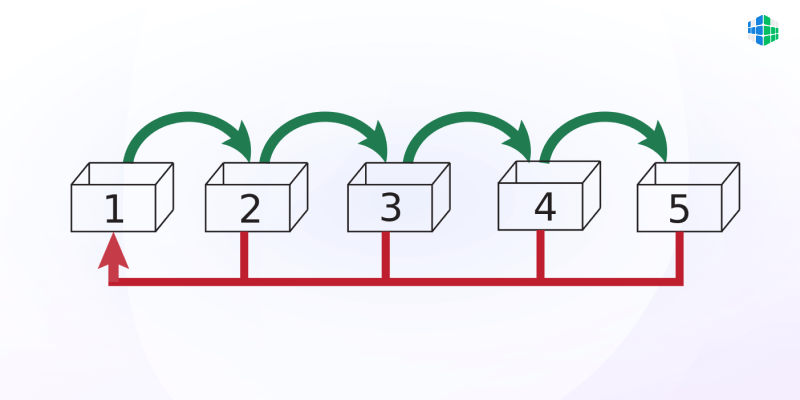
\includegraphics[width=0.49\textwidth]{img/sistema-lejtnera.png}
    \end{center}
    \caption{Система Лейтнера: 5 шагов, позволяющих выучить что угодно}
\end{wrapfigure}
Как часто вам приходится жаловаться на память? Как часто вам нужно что-то запомнить, а оно никак не запоминается? И как быстро вам надоедает все это повторять настолько, что вы решаете обойтись без этих знаний?

С подобной ситуацией сталкивается около 80\% людей, изучающих, например, иностранный язык. И как раз в помощь им была создана система Лейтнера. Однако впоследствии оказалось, что она пригодна для запоминания любой другой информации. Что же это за система такая?

\textbf{Волшебные карточки Лейтнера}

Основой системы Лейтнера являются так называемые флэш-карточки, на которых записывается информация для запоминания. Карточки могут быть обычными бумажными либо электронными.

За основу бумажной версии можно взять обычные каталожные карточки, которые можно увидеть в любой традиционной библиотеке, где есть каталоги – алфавитный, систематический, топографический. Как вариант, можно вырезать карточку удобного лично вам размера из плотной бумаги или тонкого картона.

Лайфхак для офисов и издательств – не выбрасывайте оставшиеся невостребованными карманные календарики за прошлый год. На светлом фоне можно писать черным маркером, а такие карточки будут выглядеть интереснее и веселее, чем обычные, сделанные из одноцветной бумаги.

Электронные карточки можно сделать в любом мобильном приложении для создания заметок или же воспользоваться специальным софтом. Для русскоговорящих пользователей можно рекомендовать мобильное приложение Brainscape или онлайн-программу Quizlet, также имеющую версии для iOS и Android.

Принцип использования бумажных и электронных карточек идентичен. Разница лишь в том, каким способом вы будете «тасовать колоду»: перелистывая экран или перекладывая карточки из одной стопки в другую.

\textbf{Как пользоваться карточками}

Каждый из нас замечал, что даже самое банальное «не получается» имеет свои градации: не очень получается, не всегда получается, не получается от слова «совсем». Если воспользоваться традиционным линейным способом заучивания, весь материал придется проходить каждый раз от начала до конца, будь то список новых слов по английскому, набор формул по физике или даты исторических событий.

Система Лейтнера позволяет не тратить время на повторение уже выученного материала, даже если он идет в связке с пока неизученным. Эта система удобна тем, что можно сосредоточиться только на том, что пока никак не запоминается, и регулировать частотность повторений по мере усвоения. Как это работает?



Алгоритм использования флэш-карточек:
\begin{enumerate}
    \item Распределяем весь изучаемый в данный момент материал по карточкам в режиме 1 карточка = 1 единица информации.
    \item Карточки с информацией, которую не получается запомнить совсем, складываем в первую колоду и повторяем ежедневно.
    \item Карточки с информацией, которую вы помните фрагментарно, помещаете во вторую колоду и повторяете через день.
    \item Карточки с информацией, которую вы иногда забываете или не всегда можете быстро вспомнить, помещаете в третью колоду и повторяете раз в три дня.
    \item По мере освоения материала карточки из первой колоды перекладываете во вторую, а затем в третью колоду.
\end{enumerate}

Такой подход называется методом интервальных повторений, т.е. повторений с определенными оптимальными для достижения результата интервалами. Не обязательно перечитывать всю колоду за один раз. Прочитайте столько, сколько успеваете, пока едете на работу, стоите в очереди, помешиваете кашу на медленном огне. Таких «бесполезных пятиминуток» может быть несколько в течение дня, и в сумме набегают те же 45 минут, что нужны для полноценного урока.

Теперь чуть подробнее о единицах информации. Это может быть, например, слово на английском – транскрипция – перевод на русский. Или формула по физике с расшифровкой переменных, внесенных в формулу. Или дата и название исторического события. Такой подход идеален для школьников в возрасте до 12-13 лет, которым сложно воспринимать сразу большой объем сведений.

Студенты, старшеклассники и взрослые могут расходовать площадь карточки более экономно и записывать на одну карточку сразу 2-3 связанные единицы информации. Например, три формы глагола в английском, две формулы из раздела «Кинематика» для расчета средней скорости движения и средней скорости при неравномерном движении, даты первого, второго и третьего раздела Польши в 18 столетии. Само собой, для трансфера карточки в следующую колоду нужно освоить все слова, формулы, даты с карточки.

К слову, при использовании электронных карточек вы можете получать рекомендации, сколько времени вам потребуется для запоминания той или иной информации и как часто нужно ее повторять. В частности, эта функция есть в приложении Brainscape. Вам требуется на старте самостоятельно оценить свой уровень знаний по каждой карточке от 1 до 5, и приложение выдаст свои рекомендации для дальнейшего изучения материала.

Английский, физику и историю мы взяли исключительно для примера. На самом деле, область применения карточек намного шире.

\textbf{Область применения системы Лейтнера}

Мы начали с того, что изначально данная система была разработана Лейтнером для изучения иностранного языка. Себастьян Лейтнер был журналистом, поэтому знание языков было для него профессиональной необходимостью.

Процесс изучения языка был адаптирован под существующие обстоятельства, т.е. высокую мобильность профессии журналиста, когда из-за постоянных разъездов и командировок не получается выделить фиксированное время для занятий.

Набор флэш-карточек с новыми словами, формами глаголов, местоимений, причастий, деепричастий всегда можно взять с собой. Небольшой набор легко поместится в карман мужского пиджака, а две-три стопки не займут много места в сумке. К слову, для изучения иностранных языков можно приобрести готовые карточки.

Точно так же с помощью флэш-карточек можно готовиться к экзамену по любому предмету в школе и вузе, докладу на семинаре или конференции, запоминать расположение нот и варианты аккордов на грифе гитары, разучивать длинную песню, разделив ее на куплеты, бридж и припев, а в особо сложных случаях переписав на карточки построчно.

Так же с помощью карточек можно развивать память и остроумие, поместив на них короткие шутки, анекдоты, изречения по разным поводам. Если регулярно повторять шутки и анекдоты, которые имеют свойство забываться, через какое-то время ваш мозг будет моментально реагировать на подходящую ситуацию, где можно блеснуть остроумием и выдать актуальный юмор.

Многим эта система так нравится, что они готовы заменить ею весь учебный процесс. Стоит ли это делать? Давайте подумаем.

\textbf{Система Лейтнера: в придачу или вместо?}

Тут хочется вспомнить известную поговорку: все хорошо в меру. Конечно же, система Лейтнера не может полностью заменить лекции, семинары и уроки хотя бы потому, что на семинарах и лекциях можно получить обратную связь преподавателя.

Разумеется, система Лейтнера не может заменить систематизированный курс по какой-либо специализации, будь то приемы оказания первой медицинской помощи или основы компьютерной грамотности. Карточки лишь носители единиц информации, а полностью овладеть знаниями можно, только когда вы получаете систематизированный курс лекций в нужной последовательности и учитесь применять полученные сведения на практике.

По этой же причине система не может стать альтернативой получению среднего или высшего образования, даже если на карточки перенести все формулы и даты по всем предметам. Однако система Лейтнера может существенно дополнить традиционные методы обучения, облегчить процесс усвоения и сэкономить время на изучение материала.

Как было сказано выше, пользование флэш-карточками вовсе не требует выделения фиксированного времени в вашем распорядке дня, и вы можете заполнить карточками любой пустой отрезок дня, когда не предвидится ничего более важного и интересного.

Если такой не заполненный полезными делами промежуток времени оказался слишком большим, вы можете повторить информацию из всех трех колод, а потом пойти по кругу, вернувшись к первой стопке. Это будет исключительно вам на пользу и станет отличной проверкой функциональности вашей кратковременной памяти. Вы сами сможете увидеть, с какой скоростью вы запоминаете или забываете информацию и, возможно, откорректировать методы самообразования в дальнейшем. Теперь подытожим все преимущества системы.

Преимущества системы Лейтнера:
\begin{enumerate}
    \item Простота и доступность.
    \item Возможность реализовать в бумажном или электронном формате по выбору.
    \item Возможность использования везде и всюду.
    \item Применимость для разных областей знания.
    \item Пригодность для подготовки к экзаменам по любым предметам.
    \item Пригодность для запоминания любой информации, которую можно разбить на короткие логические блоки.
    \item Развитие памяти – оперативной, среднесрочной и долгосрочной.
\end{enumerate}

К слову, с развитием памяти и техник запоминания информации вам может помочь наш курс «Мнемотехники», где вы освоите полезные лайфхаки, как быстро и надежно запоминать имена, даты, лица, термины, иностранные слова и все, что вам нужно. В качестве бонуса по окончании курса вы получите новый уровень развития ассоциативного мышления и научитесь придумывать рифмы к любым словам, требующим запоминания.

Так что желаем вам свежих знаний, полезных сведений, новой информации и ждем вас на нашем курсе, где научим все это запоминать. Поделитесь ссылкой на курс у себя на страничке в соцсетях – так вам будет легче вспомнить, где именно стоит искать этот курс, когда вы будете готовы начать учиться. Удачи!

\clearpage
\section{Метод изучения языков Китайгородской}

\textit{Источник: \url{https://4brain.ru/}}

\begin{wrapfigure}{l}{0.5\textwidth}
    \begin{center}
        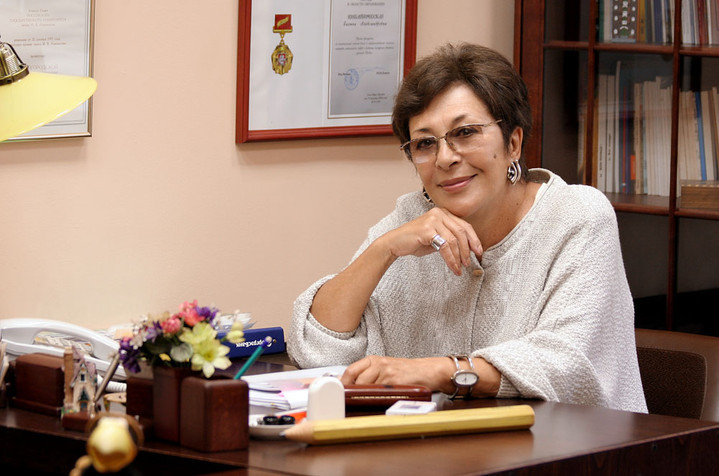
\includegraphics[width=0.49\textwidth]{img/kitaigorodskoi.jpg}
    \end{center}
    \caption{Китайгородская, Галина Александровна}
\end{wrapfigure}
С каждым днём в сфере образования появляются какие-то новые \ed{разработки}{разработка}{development}, программы, \explain{обучающие методики}{teaching methods} и другие всевозможные \ed{н\'{о}вшества}{н\'{о}вшество}{innovation}. Старые, же, или, как ещё их можно назвать, традиционные, если уж и не забываются, то просто отодвигаются на задний план по причине потери своей \ed{актуальности}{актуальность}{relevance} и малой эффективности. И эта тенденция наблюдается во всех направлениях, по которым происходит обучение, в том числе и в изучении иностранных языков.

Большинство традиционных методик обучения иностранным языкам сейчас \explain{подвергается}{undergoes; is subjected to} жёсткой критике, т.к. многие специалисты считают, что обучать им современных детей, да и взр\'{о}слых тоже, следует по ин\'{о}му пут\'{и}. А представление о прив\'{ы}чных мет\'{о}диках обучения складывается прим\'{е}рно такое:
\begin{enumerate}
    \item Огромное количество тр\'{у}дных грамматических правил, которые необходимо заучивать
    \item Десятки листов со словами, которые также нужно заучивать
    \item Объёмные неинтересные тексты, которые нужно читать, переводить и пересказывать
\end{enumerate}

Как вы сами считаете, нужно ли продолжать применять такие м\'{е}тоды в современных образовательных учреждениях? Наверняка, вы скажете, что лучше найти нечто более интересное и эффективное, что оказывало бы на учащихся большее стимулирующее воздействие, и помогало бы им гораздо быстрее осваивать лексику, грамматику и фонетику того языка, который они изучают.

И на сег\'{о}дняшний день исследователи \explain{выделяют}{identify} два основн\'{ы}х инновационных пути изучения языков, которыми являются:
\begin{enumerate}
    \item Применение методов изучения иностранных языков, осн\'{о}вывающихся на эффекте сверхзапоминания, когда восприятие и усвоение информации происходит без её критического осмысл\'{е}ния;
    \item Применение нетрадиционных методов, которые подразумевают ускоренное и максимально интенсивное обучение иностранному языку, где теоретическая база является минимальной или её вообще нет, а \explain{основной уп\'{о}р}{main emphasis} д\'{е}лается на практике, т.е. на разговорной речи в процессе жив\'{о}го общения.
\end{enumerate}

Базой об\'{о}их этих путей являются принципы суггестологии, которые б\'{ы}ли разработаны болг\'{а}рским педагогом и псих\'{о}логом Геогрием Лозановым. Ст\'{о}ит сказать, что суггестология является наукой, посвящённой раскрытию скрытого потенциала человека, и активизирующей его подсознательные ресурсы. В качестве примера можно назвать м\'{е}тод всем известного «25 кадра», а также обучение во сне. И как раз одним из м\'{е}тодов обучения иностранным языкам, которые основываются на принципах суггестологии, является метод Галины Александровны Китайгородской.

\textbf{Метод Г. А. Китайгородской}

Метод Г. А. Китайгородской, который также называют м\'{е}тодом «Активизации рез\'{е}рвных возможностей личности и коллектива», нельзя назвать новым, т.к. он был разработан свыше 35 лет назад, однако он считается исключительно \ed{нов\'{а}торским}{нов\'{а}торский}{innovative} и уже ставшим классическим в области интенсивного обучения.

Важно также сказать, что именно Галиной Александровной Китайгородской была создана единственная в России научная система интенсивного обучения иностранным языкам, а также был введён сам термин «интенсивное обучение». И с момента создания этой системы её эффективность была оценена огромнейшим количеством людей, которые в рек\'{о}рдно короткие сроки овладели иностранными языками.

Отличие м\'{е}тода Китайгородской от традиционных заключается в том, что он \explain{з\'{и}ждется}{is based on} на психологических резервах личности и коллектива при \ed{целенаправленной}{целенаправленный/-ая}{purposeful; targetted} манипуляции социально-психологическими процессами \ed{межличностного}{межличностный}{interpersonal} группового взаимодействия, благодаря чему учащиеся за совершенно мизерное время очень легко и продуктивно перерабатывают большие объёмы новых знаний.

Ключевое место в системе интенсивного обучения занимает термин «активизация» --- процесс, который направлен на достижение человеком активности и стабилизацию данного состояния. В своей изначальной интерпретации понятие «интенсивность» рассматривается как «напряжённость», а именно: состояние активности в конкретный момент времени. Точно также следует и трактовать понятие «интенсивного обучения» в рамках системы Г. А. Китайгородской – оно должно пониматься как динамизм, активное взаимодействие педагогов и группы учащихся, учащихся друг с другом, активизация процессов \ed{познания}{познание}{knowledge; cognition}, ресурсов памяти, воображения и внимания.

Тот ученик, который устал, засыпает на занятиях и нисколько не заинтерес\'{о}ван в своём обучении, не способен \explain{надлеж\'{а}щим \'{о}бразом}{properly} воспринимать большие объёмы информации и \explain{всецело}{wholly; entirely} отдаваться общению со своими партнёрами по обучению. А методика Китайгородской спос\'{о}бна привести учащегося в такое состояние, в котором он будет максимально \explain{\'{у}мственно}{mentally} и нередко даже физически активен, по причине чего будет обесп\'{е}чен самый высокий показатель интенсивности процесса обучения. Если говорить несколько проще, путь овладения человеком иностранным языком, согласно системе Китайгородской, очень \explain{схож}{similar} с тем путём, идя по которому ребёнок осваивает свой родной язык.

Сначала учен\'{и}к двигается вперёд по различным стадиям формирования способности к речи, начиная с интонационной, затем переход\'{я} к лексико-грамматической, а после --- к синтаксической и фонетической. Причём, происходит всё это совершенно естественным образом, а не наоборот, как это можно наблюдать в традиционных м\'{е}тодах обучения. И сроки овладения новым навыком значительно сокращаются.

Уже в процессе первого занятия ученик начинает \explain{изъясняться}{(here) to speak} на иностранном языке при помощи готовых конструкций. \ed{Изначально}{изнач\'{а}льно}{initially} он, конечно, не знает правил грамматики, но постепенно переходит на уровень анализа тех конструкций, которые применяет, а потом снова начинает использовать их в своей речи, вместе с этим производя решение всевозможных задач в атмосфере естественного общения, но уже на совершенно другом уровне. Это называется микроциклом. И уже только на одном этапе процесса обучения этих микроциклов присутствует масса. В итоге ученик осваивает несколько тысяч лексических единиц в течение одного курса, но наиболее важно то, что он научается легко и непринуждённо применять их в различных ситуациях общения.

Всего за восемь недель обучения учащиеся начинают изъясняться на иностранном языке, снимают языковые барьеры, раскрепощаются и получают мощнейшую мотивацию к дальнейшему освоению языка. И этому в немалой мере способствуют специализированные учебники, предназначенные для каждого конкретного языка и каждого уровня обучения, должным образом организованное взаимодействие в группе учеников, атмосфера дружелюбия и творчества, интересные для выполнения задания, которые вызывают у учащихся желание их выполнять, уникальный психотерапевтический эффект, к достижению которого стремятся педагоги Школы Китайгородской, и множество других \ed{немаловажных}{немаловажный}{important} факторов.

\explain{В дополнение к этому}{In addition to this}, следует сказать, что с\'{о}зданная более 35 лет назад Галиной Александровной Китайгородской система обучения иностранным языкам в настоящее время актуальна и \explain{востр\'{е}бована}{in demand} гораздо больше, чем когда-либо вообще. И в качестве заключения несколько слов о Школе Китайгородской.

\textbf{Школа Китайгородской}

Школа Китайгородской является единственным в нашей стране научно-образовательным центром, в котором научные и практические м\'{е}тоды напр\'{а}влены на достижение единого результата --- интенсивного обучения людей общению на иностранных языках.

Данное научно-образовательное учреждение было основано в 1985 году на базе открывшегося в 1979 году при Московском государственном университете им. М. В. Ломоносова Центра интенсивного обучения иностранным языкам.

Сегодня в Центре интенсивного обучения иностранным языкам пров\'{о}дится обучение для студентов и преподавателей МГУ им. М. В. Ломоносова, а в самом научно-образовательном центре «Школа Китайгородской» имеют возможность проход\'{и}ть обучение все, кто желает овладеть иностранными языками.

И уникальность Школы Китайгородской заключается вот в чём:
\begin{enumerate}
    \item Только в Школе Китайгородской иностранные языки преподаются по \'{а}вторской мет\'{о}дике интенсивного обучения, разработанной Г. А. Китайгородской, защищённой докторской диссертацией и описанной многими монографиями, методическими пособиями и статьями.
    \item Система интенсивного обучения Г. А. Китайгородской \ed{снабжен\'{а}}{снабжён, снабжен\'{а}}{is equipped} \'{а}вторскими учебниками, специально разработанными для каждого из уровней.
    \item Преподавательский \explain{сост\'{а}в}{staff} Школы Китайгородской \explain{состо\'{и}т из}{consists} лучших учеников-последователей профессора Г. А. Китайгородской, которые великолепно владеют мастерством педагогики.
\end{enumerate}

Школа Китайгородской всегда верна своей специфике и сохраняет неизменное высшее качество обучения иностранным языкам, которое основано на многолетнем опыте, множестве экспериментов и исследований.

\clearpage

\section{Активизация возможностей личности и коллектива}

\textit{Источник: \url{https://kitaygorodskaya.ru/method}}

М\'{е}тод «Активизация возможностей личности и коллектива» (Метод Китайгородской) --- это уникальная система обучения, защищённая д\'{о}кторской диссертацией, оп\'{и}санная в монографии, метод\'{и}ческих пос\'{о}биях и стать\'{я}х. Это инновация, ставшая классикой интенсивного обучения.

В течение многих лет нашей научной базой являлся Центр Китайгородской в МГУ им. М.В. Ломоносова.
Несколько десятков лет наш Метод работает на обучение жив\'{о}й разговорной речи. Уникальность Метода Китайгородской состо\'{и}т в том, что благодаря научно разработанной системе, используемым техникам запоминания и специально созданным учебникам результат достигается в кратчайшие сроки.

\textbf{Что же такое интенсивное обучение?
}

Чтобы точно определить, что является для нас главным в концепции так называемого интенсивного обучения, следует ввести слово «активизация». Активизация --- процесс, направленный на достижение активности личности и сохранение этого состояния. В своем исходном значении\footnote{in its original meaning} слово «интенсивный» (лат. "intensus") означает «напряжение», т.е. активность в единицу времени. В этом случае понятие «интенсивное обучение» соответствует нашей концепции --- динамизм, активность во взаимодействии преподавателя и уч\'{е}бной группы, учащихся между собой. Именно состояние активности преподавателя и учащегося обеспечивает высокий уровень интенсивности (активности) учебного процесса.

Подобное представление об обучении исключительно актуально, так как проблемы взаимодействия людей \explain{всё более}{more and more} \explain{прочно}{firmly, substantially} сращиваются с проблемами обучения иностранным языкам. Ведь сегодня стратегической целью обучения является не только овладение языком как средством общения, но и языком как средством \ed{приобщения}{приобщение + \textit{к}}{familiarisation} к иной культуре. Социопсихолингвистические исследования за рубежом и в нашей стране позволяют \explain{принимать за точку отсчёта}{take as a starting point} не языковой код, а речевую активность, активность речевой д\'{е}ятельности. Те\'{о}рия коммуникации \explain{убеждает}{convinces} нас в том, что недостаточно знать язык, систему языка, правила функционирования языкового кода. Чтобы общаться, надо знать, как п\'{о}льзоваться языком в определённом контексте, т.е. выучить язык означает сегодня овладеть речевым поведением в естественных ситуациях. В этих условиях функции языка, а не его структура, приобретают первостеп\'{е}нное значение в процессе обучения.

В нашей концепции интенсивного обучения мы рассматриваем овладение иноязычным общением в его устной и письменной форме с социально-психологических позиций. Общение на изучаемом языке \explain{прон\'{и}зывает}{pervades} процесс обучения, являясь одноврем\'{е}нно целью этого обучения, основным средством и условием его достижения. Поэтому интенсивное обучение может быть определен\'{о} как особым образом организованное обучающее общение, в ходе которого происходит \explain{уск\'{о}ренное}{accelerated} \explain{усвоение}{assimilation} материала (овладение предметом) и активное \explain{совершенствование}{improvement}, развитие личности (учащихся и преподавателя).

Естественно, что такое понимание интенсивного обучения исключает представление о «минимизации» учебного материала, а также усилий преподавателя и учащихся. В нашем случае речь иёт о максимизации объёмов учебного материала и усилий преподавателя и обучаемых, т.к. интенсивное обучение основано на активизации их деятельности. Активность участников учебного процесса выражается в максимальной и постоянной их вовлечённости в процесс управляемого группового взаимодействия, общения-обучения.

Широкое использование группов\'{ы}х (коллективных) форм взаимодействия в уч\'{е}бном процессе приводит к тесному \ed{переплетению}{переплет\'{е}ние}{weave; interlacing} методики и социальной психологии, что характеризует нашу концепцию интенсивного обучения. Это единственная психолого-педагогическая концепция, которая строит учебный процесс на основе принципа коллективного взаимодействия, «социального взаимодействия». Именно поэтому единицей организации учебного материала и учебной деятельности является ситуация взаимодействия, динамическое событие, моделирующее образы реальной жизни.

Итак, мы предлагаем иной психологический путь достижения педагогической цели. Психологические опоры интенсивного обучения требуют соответствующей организации учебного материала и учебного процесса.

Для более полного представления об интенсивном обучении необходимо остановиться на психолого-педагогических пр\'{и}нципах, которые не только характеризуют его, но и помогают преподавателю творчески использовать предлагаемое учебное пособие, оставаясь в рамках метода активизации возможностей личности и коллектива.

\textbf{Пр\'{и}нцип личностного-ориентированного общения}

Слово «общение» понятно всем, но может быть именно поэтому, когда это слово употребляется применительно к организации учебного процесса, то подчас возникает \explain{недоумение}{confusion; perplexity}: общение преподавателя с учениками, а тем более общение учеников между собой очень похвально, но на уроке мало времени, это слишком большая роскошь. Да и вообще, какое отношение имеет общение к обучению?

Попробуем ответить на этот вопрос с научной точки зрения. \explain{Общеизвестно}{It is generally known}, что личность формируется и функционирует в постоянном взаимодействии с другими людьми в основных видах деятельности: игр\'{е}, учёбе, труд\'{е}. Развитие личности учащегося протекает в двух взаимосвязанных деятельностях: учебной и общении. Известно также, что гармоничное развитие личности \explain{во многом}{in many ways} обеспечивается единством этих видов деятельности. Тенденция к \explain{слиянию}{merger} процессов обучения и общения характеризует современную педагогику и психологию обучения. \ed{Благоприятные}{благоприятный}{favourable} условия для достижения эффективных результатов открываются тогда, когда требования учебной задачи представляются обучаемому привлекательными, удовлетворяющими его потребности.

Чтобы создать необходимые для этого условия, надо построить учебный процесс таким образом, чтобы отношение к изучаемому предмету формировалось через отношение к другому человеку (соученику, учителю), а оно, в свою очередь --- через групповое взаимодействие, иными словами, необходимо обеспечить максимальное слияние общения и обучения. Именно в этом случае, по утверждению психологов, общение выполняет обучающую и развивающую функции и приводит к наиболее продуктивному овладению изучаемым предметом при одновременном всестороннем личностном развитии. Все это, как нам кажется, дает основание для введения понятия обучающего общения.

\textit{Почему же мы формулируем этот принцип как принцип личностного общения?}

Прежде всего, в понятие «личностное» мы вкладываем психотерапевтическое и психологическое содержание: \explain{доверительность}{confidence}, поддержка, \explain{доброжелательность}{kindness; benevolence}. Ведь общение, диалогическое общение, с позиции социальной психологии подразумевает установление отношений взаимного доверия, откровенности. В диалоге (в широком смысле слова) представлены голоса всех его участников, что позволяет \explain{сопоставлять}{compare; contrast; juxtapose} различные точки зрения, определять свою собственную и рассматривать ее как одну из возможных.

Диалогическое общение в таком расширительном понимании предполагает организацию особого типа отношений его участников, характеризующихся \ed{устремлённостью}{устремлённость}{aspiration; tendency; desire} к другому человеку, вниманием и интересом к нему, способностью \ed{дорожить}{дорожить кому-то}{высоко ценить что-либо, придавать большое значение чему-либо} другим человеком, видеть в нем цель, а не средство. Взаимный характер общения приводит к активной позиции каждого его участника. Однако надо помнить, что одно из важнейших умений в общении --- умение слушать собеседника. Для преподавателя интенсивного обучения это особо важное качество, т.к. он должен уметь строить общение в учебной группе по типу реального общения, «вплетая» в этот контекст неформального личностного общения учебный материал (упражнения).

\textit{Принцип личностного общения.}
Реализация этого умения на практике означает, например, что, задав вопрос, преподаватель должен уметь выслушать своего ученика не только и не столько как «ученика», но и как собеседника, партнера. Это умение \explain{проявляется}{is manifested} в реакции на содержание, смысл сказанного учеником.

Преподаватель не стремится оценить ответ ученика, что так привычно в педагогической практике. Он выражает, высказывает свое отношение к содержанию сообщения. Это невероятно важно, т.к. именно выражение своего отношения к сказанному учеником выводит эту учебную ситуацию за рамки формального взаимодействия, превращает учебное общение в неформальное личностное, т.к. позволяет «вплести» тренировку учебного материала (упражнения) в контекст реального общения.

Организация такого обучающего общения требует от преподавателя специальных умений и определенных усилий, особенно на начальном этапе, когда ученик еще очень ограничен в выборе языковых средств и, кроме того, в сознании учащегося (да и преподавателя) действует стереотип учебного взаимодействия, созданный предшествующим опытом учения и преподавания. Этот стереотип держит преподавателя в рамках «опросной» системы, когда любой ответ, сообщение ученика замыкается на преподавателя, ответ которого заключает в себе оценку формальной стороны сообщения ученика. Необходимо сразу же преодолевать этот стереотип, и с этой точки зрения чрезвычайно важным оказывается использование специального приема, который мы называем «передачей», «перепасовкой» реплики (ответа, сообщения) одного учащегося другим (группе), стимулируя тем самым их собственные высказывания, реакции, активность в поддержании и развитии диалога в группе. Преподаватель \explain{ос\'{о}знанно}{consciously} стремится не принимать все реплики учащихся «на себя», отдавать их, как мяч в волейболе.

\textit{Как организовать личностное общение?}

Успешность в организации личностного общения на занятиях зависит от того, как \explain{отобран}{selected $<$ отбирать/отобрать: to choose; to select; to single out} и организован учебный материал. Так, например, отбор учебного материала обязательно предусматривает наличие специальных языковых средств для вступления в контакт, для выхода из контакта и т.п., всего того, что позволяет обучаемому выражать себя как личность в организованном и управляемом преподавателем иноязычном общении. Организация учебного материала в жизненно значимых ситуациях, комбинации которых заложены в текстах-полилогах, служит моделью личностного общения, помогая обучаемому в дальнейшем находить речевые способы и средства решения многих других однотипных ситуаций, отталкиваясь от имеющегося образца.

Не только отобранный учебный материал, представленный в текстах-полилогах, не только система коммуникативных упражнений, основой которой является принцип личностного общения, но и такие характеристики, как количество обучаемых, состав группы и ее пространственное расположение, подчинены принципу личностного общения. Оптимальный объем группы --- 12 человек, состав гетерогенный, что позволяет создать в группе репрезентативную модель общества, расположение в аудитории --- полукругом, лицом к лицу. Эти параметры, кстати, характерны для всех групповых форм психологической работы (Т-группы, группы тренинга умений, психодрама и т.д.).

\textbf{Принцип игровой/ролевой организации учебного материала и учебного процесса}

Наблюдения за учебным процессом в средней и высшей школе, особенно за обучением иноязычному общению, показывают, что одна из серьезных причин очень малой эффективности заключается в низком уровне мотивированности обучаемого. Большей частью преподаватель предлагает учащимся псевдокоммуникативные задания типа: «Пригласите соседа в гости», «Узнайте, как доехать до...». Речевые действия учащихся при выполнении подобных заданий не мотивированы, и значит --- формальны. Эти задания не многим отличаются от заданий типа: «Перескажите текст», «Переведите предложение» и т.п. В них нет ответа на главный вопрос, возникающий у обучаемого, --- «Зачем, с какой целью я должен это сделать, сказать?».

\textit{Принцип ролевой организации.}
Вероятно, для \explain{устранения}{elimination} этого недостатка следует прежде всего осознать важное место ролевого поведения в учебной деятельности учащихся. Опыт интенсивного обучения иностранным языкам позволяет \explain{сделать вывод}{to draw a conclusion} о больших возможностях ролевого общения (ещё далеко не полностью исследованных) и целесообразности его использования в обучении.

Эта идея поддерживается лингвистами, которые видят в ролевом общении эффективный способ приобретения речевой компетенции, и психологами, \explain{утверждающими}{которые утверждают $<$ утверждать/утвердить: to assert, to argue, to allege, to state; to claim; to approve. Here: ``who argue''}, что приёмы организации ролевого общения напр\'{а}влены на приведение в действие механизмов мотивации. Ролевое общение на иностранном языке в условиях интенсивного обучения --- это не фрагмент занятия, не методический прием, не упражнение, а основа построения учебного процесса. Обучать иноязычному общению (в его устных и письменных формах) можно лишь в \ed{непрерывном}{непрерывный}{continuous, uninterrupted} личностно-ролевом взаимодействии.

Ролевое учебное общение в интенсивном обучении предполагает постоянную активность субъектов общения (всех учащихся и преподавателя), которые не ограничиваются просто восприятием сообщения и реакцией на него, а стремятся выразить свое отношение к полученной информации. Специфика ролевого учебного общения заключается в том, что оно сохраняет все социально-психологические характеристики истинного общения. Поэтому общение является для обучаемого целью его речевого (или неречевого) действия в условиях, максимально приближенных к неучебной \ed{совместной}{совм\'{е}стный}{joint} деятельности. Для преподавателя же это общение является и учебным, поскольку ситуации общения (упражнения) им планируются и организуются.

Преподаватель управляет общением при решении конкретных учебных задач, необходимых для реализации целей курса обучения. Таким образом, с позиции преподавателя, ролевая игра, ролевое общение --- форма организации учебного процесса, а с позиции учащихся --- коммуникативная, познавательная, игровая деятельность. Увлеченный решением сменяющих друг друга коммуникативных задач в общении с различными партнерами, обучаемый большей частью не осознает учебной стороны решаемых задач. Исключение составляют чисто познавательные, аналитические задачи, но и они преподносятся в форме, поддерживающей интерес учащихся. Организованная как личностное общение, учебная деятельность протекает в форме общения-игры.

Важно \explain{напомнить}{to remind}, что игра понимается нами в широком смысле слова --- как форма \ed{непосредственного}{непосредственный}{direct, immediate}, но \ed{продуманного}{продуманный}{well thought-out} и управляемого общения преподавателя и группы. Кстати, неправильное понимание игры --- одна из причин больших трудностей при овладении профессией преподавателя интенсивного обучения.

\textit{Что же такое игра?}

На этот вопрос наиболее \explain{чётко}{clearly} отвечают психологи, определяя игру как важный тип и уровень функционирования личности взрослого человека, как условие сохранения его психического здоровья и \ed{полноценной}{полноценный}{full-fledged} \explain{созидательной}{созидательный}{creative, constructive} деятельности. Главное, чтобы предлагаемые ролевая игр\'{а}, ролевое общение были по своему содержанию на соответствующем обучаемому контингенту интеллектуальном уровне. К сожалению, примитивное понимание преподавателем игры, игровой деятельности иногда приводит к «детским играм», примитивным коммуникативным задачам, т.е. к снижению интеллектуального творческого уровня обучения.

\textit{Как же преподаватель организует ролевое общение и управляет им?}

Прежде всего, преподаватель организует непрерывное общение через решение множества коммуникативных задач, представленных в коммуникативных упражнениях. При подготовке к занятию преподаватель создает упражнения для решения конкретных учебных задач на определенном языковом и речевом материале, а затем комбинирует их в сценарии занятия. Коммуникативные задания в упражнениях формулируются как естественные жизненные ситуации, исходя из конкретного языкового и речевого материала, который запланирован преподавателем для определенного этапа его отработки.

Принцип ролевой организацииТрудно переоценить методическое значение роли. Роль является одним из главных средств обеспечения мотивированных многократных повторений учащимся одних и тех же языковых и речевых единиц, что необходимо для формирования речевого навыка. Но и психологическое, психотерапевтическое значение роли огромно.

Учащийся в зависимости от типа своей личности, от степени владения изучаемым языком, от конкретной роли в данной ситуации может «самовыражаться», творчески реализовывать свои знания, умения, свой интеллектуальный потенциал, а может «прятаться за свою роль», т.е. минимальными языковыми средствами и, как правило, широко привлекая невербальные средства, «создавать свою роль» как средство защиты. Преподаватель же продуманно \ed{вовлекает}{вовлекать/вовлечь}{to involve} каждого в общую деятельность, распределяет роли в ситуации, делает временным лидером каждого, одним словом, управляет общением, учит общаться.

Роли-легенды, заложенные в тексте-полилоге, и ситуации полилога реализуются в учебном процессе лишь при введении текста-полилога и, частично, на первом занятии тренировки в общении. На всех остальных занятиях преподаватель «работает» на ситуациях-вариантах при использовании самых различных ролей и масок, что позволяет отрабатывать необходимый языковой и речевой материал в большом количестве разных ситуаций.

Постоянная смена ролей и ситуаций на занятиях способствует поддержанию мотивации речевых действий учащихся при большом количестве повторений одних и тех же языковых единиц и грамматических явлений, что является необходимым условием для формирования прочного и \ed{гибкого}{гибкий}{flexible} речевого навыка. Третий принцип --- коллективное взаимодействие --- основной психологический принцип, на котором построено интенсивное обучение. Суть его --- организация групповых (коллективных) действий, способствующих внутренней мобилизации возможностей личности обучаемого.


\textbf{Принцип коллективного (группового) взаимодействия}

Принцип коллективного взаимодействия определяет такой способ организации учебного процесса, при котором:
\begin{enumerate}
    \item учащиеся активно общаются друг с другом, обмениваясь учебной информацией, расширяя за счет этого свои знания, совершенствуя умения и навыки;
    \item между участниками складываются благоприятные взаимоотношения, служащие условием и средством эффективности обучения и творческого развития каждого;
    \item условием успеха каждого является успех остальных.
\end{enumerate}

Таким образом, активное общение преподавателя с учащимися и учащихся между собой является социально-психологическим фактором успешности процесса обучения, одновременно обеспечивая эффективность формирования познавательных действий и приемов общения на изучаемом языке. Совместные действия и межличностные отношения в системе учитель-ученик, ученик-группа и т.д. являются также средством повышения продуктивности индивидуальной деятельности ученика.

В активном взаимодействии друг с другом учащиеся не только обмениваются знаниями о системе языка, когда, помогая друг другу, дают языковые комментарии, объясняют правила своему партнеру, но и учатся общаться. Процесс обучения иноязычному речевому общению --- это двусторонний процесс, в котором многое приобретает не только учащийся, но и учитель.

Организуя иноязычное общение и управляя им в группе, он совершенствует свои коммуникативные умения. В ходе взаимодействия с учащимся \explain{уточняется}{refines} его собственное \explain{представление о себе}{self image}, становится более адекватной самооценка.

\textbf{Типы учебного взаимодействия }

Особую значимость приобретает вопрос о типах учебного взаимодействия. Типы и способы учебного взаимодействия должны обеспечивать постоянную и активную \explain{вовлечённость}{involvement} учащихся в процесс обмена информацией. В нашей методической системе используются многие способы учебного взаимодействия, дополняющие друг друга и придающие учебной деятельности коллективный характер: одновременная работа в парах (диадах); одновременная единая или дифференцированная работа в триадах; одновременная единая или дифференцированная работа в микрогруппах по 4 человека; работа в командах (2 микрогруппы); учащийся-группа; преподаватель-группа; преподаватель-микрогруппа и т.д.

В интенсивном обучении чрезвычайно усиливается активность учащегося, так как на протяжении всего занятия он решает попеременно с другими учениками поступающие одну за другой от преподавателя коммуникативные задачи. В результате, благодаря его усилиям, сознательно регулируемым преподавателем, конструируется такая система отношений, которая позволяет как можно полнее раскрыть, использовать и развить возможности каждого.

Развитию творческой индивидуальности обучаемых в коллективной учебной работе способствуют:
\begin{enumerate}
    \item \explain{доверительные отношения}{trusting relationships} между преподавателем и учащимися, которые освобождают учащихся от \ed{скованности}{ск\'{о}ванность}{(lit) inhibition; stiffness} и чувства неуверенности в себе;
    \item поощрения со стороны преподавателя и товарищей по группе, помогающие обучаемому поверить в свои силы;
    \item идентификация обучаемого с группой;
    \item организация учебной деятельности в совместных игровых формах;
    \item организация учебной деятельности в форме серий заданий, интересных для обучаемых и предполагающих их активное взаимодействие.
\end{enumerate}

\textbf{Роль преподавателя }

Организация речевого общения в условиях коллективной познавательной деятельности предполагает особую роль преподавателя. Речь идет о таком типе педагогического общения, который \explain{бл\'{и}зок к}{close to} оптимальному --- развивающему и \ed{взаимообогащающему}{взаимообогащающий $<$ обогощать/обогатить (\textit{что, чем}): to enrich (e.g., обогащать ум знаниями)}{mutually enriching} человеческому общению. Поэтому понятие профессионализма преподавателя требует \ed{пересмотра}{пересмотр}{revision}, включения в него особых педагогических способностей, связанных с реализацией коллективных форм сотрудничества как преподавателя с обучаемым, так и обучаемых между собой.

Вероятно, наш метод по своей методологической природе более элитарен по отношению к педагогам, \ed{предъявляя}{предъявляя}{presenting (предъявлять)} повышенные требования к их профессиональным и человеческим качествам. Ну что ж? Может быть и хорошо, что преподавать по этому методу не каждый сможет.

Коллективная познавательная деятельность, а также демонстрируемые преподавателем формы поведения, способствующие созданию атмосферы доброжелательности, взаимопомощи, внимательного отношения к партнерам, создают оптимальные условия для активизации возможностей каждого учащегося и развивают способность правильно воспринимать других и адекватно оценивать себя, свои \ed{поступки}{поступок}{action}, результаты своей деятельности.

Постоянное учебное взаимодействие с меняющимися партнерами дает возможность каждому правильно увидеть себя, оценить, прогнозировать поведение. На фоне положительной установки на восприятие каждого члена группы, которая сохраняется и развивается в ходе обучения, процесс формирования адекватной самооценки и уровня притязаний протекает быстрее.

\textbf{Принцип концентрированности в организации учебного материала и учебного процесса}

Концентрированность учебных часов является одной из внешних характеристик интенсивного обучения. Однако наличие этой характеристики еще не означает, что данное обучение --- интенсивное. Понятие концентрированности должно быть расширено, что позволит детерминировать специфику интенсивной системы обучения. В условиях интенсивного обучения, когда решаются задачи обучения устным и письменным формам иноязычного общения, как правило, за минимальные сроки, оказываются принципиально важными еще два фактора: количество (объем) учебного материала и его \explain{распределение}{distribution} в курсе обучения.

Увеличение объема учебной информации в курсе, \explain{предпринятое}{{undertaken}} ещё Г. Лозановым\footnote{Георгий Лозанов: болгарский педагог и психолог, разработавший в 1960-е годы метод суггестопедии, используемый для ускоренного обучения иностранным языкам.}, \explain{обусловлено}{is due to}, на первый взгляд, чисто внешними обстоятельствами --- \ed{сжатыми}{сжатый}{compressed} сроками обучения. Но такое понимание причин увеличения и концентрации материала было бы несколько \explain{упрощённым}{упрощённый}{simplified}. По с\'{у}ти, речь идёт о взаимозависимости двух факторов. С одной стороны, открывшиеся возможности активизации учебной деятельности создали предпосылки для успешного усвоения повышенных объемов концентрированной учебной информации. С другой стороны, концентрированность учебного материала оказывает активизирующее воздействие на познавательные процессы. Обучаемый как бы перестраивается на новый, более активный режим деятельности, который способствует максимальным \ed{проявлениям}{проявление}{manifestation} его творческих возможностей, в частности, возможности запоминать большие объемы информации без специального заучивания.

Концентрированность в организации учебного материала и учебного процесса находит своё \explain{воплощение}{embodiment} в предлагаемой нами трёх\'{y}ровневой модели овладения устными и письменными формами иноязычного общения «Синтез-Анализ-Синтез». Этапы овладения учащимися иноязычным общением по данной модели непосредственно связаны с объемом учебного материала и его распределением в курсе обучения.

При определении общего объема учебного материала мы исходим из максимума, необходимого для реализации целей курса обучения (в нашем случае 2000-2500 лексических единиц).

\textit{Первый этап} (С1) предполагает формирование у обучаемых коммуникативного \ed{ядр\'{а}}{ядр\'{о}}{core, nucleus},
практически обеспечивающего устные формы общения на относительно простом уровне. Для решения этой задачи необходимо овладение значительным объемом языкового материала (800-1200 л.eд.).
Большой объем учебного материала, сконцентрированный на первых семи-десяти занятиях курса, необходим для дальнейшего плодотворного осмысления учащимися
\explain{накопленного}{накапливать/накопить: to accumulate; накопленный: accumulated} ими речевого опыта, систематизации языковых явлений, т.е. следующего этапа --- анализа.
Именно большой объём материала, усвоенный на первом этапе обучения, создаёт базу для последующей самостоятельной аналитической д\'{е}ятельности учащихся и обеспечивает сравнительную лёгкость её протекания. \ed{Следует оговорить}{следует оговорить}{it should be specified},
что начальный этап обучения проходит в устной форме, т.е. без полной и постоянной зрительной опоры на текст (даже если обучаемые не «нулевого» уровня). \ed{Обильное}{обильный}{abundant} слушание, происходящее на этом этапе, развивает фонематический слух учащихся, языковую догадку, дает возможность обучаемому \explain{опознавать}{to identify, to recognise, to spot} в речи языковые формы в их оппозиции, в сопоставлении и различном окружении, что одновременно активизирует аналитические процессы.
Нельзя \explain{упускать из виду}{overlook} и ещё одно важное следствие: поступление больших объёмов учебного материала. Оно даёт возможность преподавателю организовывать ситуации, максимально приближенные к реальному общению, на первом же занятии, и тем самым с самого начала создавать высокую мотивацию учения.

\textit{Этап Анализа}, как \explain{промежуточный}{interim} этап, предполагает поступление меньших объёмов новой учебной информации, чем на этапе Синтез.

Однако, по сравнению с принятыми в практике обучения нормами, объём поступающей на этапе Анализа информации остаётся высоким. Материал продолжает поступать в концентрированном виде (большое количество новой учебной информации за одно предъявление). Этот этап необходим для перехода от репродукции речевых высказываний в данной ситуации и для данных целей (С1), к их активной продукции и ситуативному варьированию (С2). Третий этап предполагает поступление больших объемов лексической информации при практическом отсутствии нового грамматического материала.

Концентрированность в организации учебного материала, естественно, \explain{предопределяет}{determines} концентрированность в организации учебного процесса. Имеющиеся в тексте ситуации являются основой для множества других, которые включаются в коммуникативные упражнения для тренировки каждого лексико-грамматического явления на разных уровнях его отработки. Сменяя друг друга, вариативные упражнения создают насыщенность, «плотность общения» на занятии, обеспечивая постоянную речевую активность всех участников общения, всей учебной группы. А это, в свою очередь, позволяет\footnote{позволяет + кому} учащимся усваивать большие объемы материала.

Принцип концентрированности в организации учебного материала и учебного процесса недостаточно полно определял бы интенсивное обучение иностранным языкам, если бы мы не дополнили его понятием коммуникативной связанности. Коммуникативная связанность, которая понимается нами как интегрирующая функция коммуникативного взаимодействия, позволяет обеспечить овладение учащимися большими объемами материала, создавая легкость в восприятии новых учебных текстов, снимая монотонность и поддерживая мотивацию при отработке большого количества лексико-грамматических явлений. Коммуникативные связи --- это прежде всего смысловые связи. Именно текст-полилог, определяющий благодаря ролевой структуре взаимодействие участников коммуникации, в наибольшей степени насыщен коммуникативными связями, которые, в частности, выявляются в его лингвистических характеристиках.

Эти связи заложены в каждом новом учебном тексте-полилоге и проявляются в сюжете, который объединяет всю макроситуацию, раскрывающуюся в большом количестве (от 5 до 10) микроситуаций, связанных по смыслу и естественно вытекающих одна из другой в рамках правил коммуникации. Это позволяет учащемуся не только прогнозировать появление каждой следующей микроситуации, не только догадываться о каждой последующей реплике, но и создает смысловую коммуникативную канву, способствующую запоминанию всего текста-полилога.

Что же касается коммуникативной связанности в организации учебного процесса, то она обеспечивается контекстом общения преподавателя с группой. Именно контекст объединяет все упражнения, отобранные для одного занятия, в единое смысловое целое. Иначе говоря, создается сценарий занятия, который, как правило, не просто повторяет, а развивает в серии упражнений сюжет учебного текста. При этом преподаватель разрабатывает множество конкретных вариантов тех микроситуаций, которые заложены в учебном тексте, затем располагает их в определенной последовательности, диктуемой учебными задачами занятия, и, наконец, включает их в смысловой коммуникативно \explain{значимый контекст}{significative/meaningful context} своего общения с учебной группой. Таким образом, понятие коммуникативной связанности дополняет понятие концентрированности в организации учебного материала и процесса обучения.

\textbf{Принцип полифункциональности учебной деятельности и упражнений}

И, наконец, пятый принцип отражает специфику организации учебного процесса согласно модели овладения иноязычным общением (С1—А—С2). Это --- принцип полифункциональности упражнений. Данный принцип тесно связан с предыдущим, так как концентрированность и коммуникативная связанность в организации учебного материала и учебного процесса определяют специфику коммуникативных упражнений, а именно — их полифункциональность.

Полифункциональность упражнений соответствует тому подх\'{о}ду при обучении иностранному языку, который предполагает одновременное и параллельное овладение языковым материалом и речевой деятельностью, в отличие от традиционного подхода, предусматривающего последовательное овладение сначала языковым материалом, а затем --- речью. Поскольку приобретение навыков и умений иноязычного общения возможно лишь через непрерывное общение в ситуациях, моделирующих реальную коммуникативную деятельность, то единственно возможным в условиях интенсивного обучения является первый подход. Он описывается предлагаемой нами моделью овладения иноязычным общением (С1—А—С2).

На основе данной модели построена система упражнений-взаимодействий преподавателя и учащихся, учащихся между собой, опосредованных иноязычным материалом и определенными межличностными отношениями участников общения. Каждое коммуникативное упражнение одновременно решает несколько задач, представленных в определенной иерархической последовательности для каждого данного этапа обучения и данного этапа занятия.

Принцип полифункциональности упражнений строится на том, что выражение какого-либо коммуникативного намерения предопределяет выбор соответствующих грамматических форм, а каждая данная грамматическая форма требует адекватного для нее лексического наполнения. В организации упражнений это отражается следующим образом: тренировка употребления каждой данной грамматической формы осуществляется в серии упражнений, где в меняющихся ситуациях реализуется одно и то же коммуникативное намерение (например, сомнение можно выражать по разному поводу, в разных обстоятельствах, в разных ролях). При этом для учащегося любое упражнение монофункционально --- он решает коммуникативную задачу. Для преподавателя оно всегда полифункционально, так как он осознает необходимость решения нескольких задач в одном упражнении:
\begin{enumerate}
    \item тренировки в решении какой-либо коммуникативной задачи;
    \item тренировки в употреблении грамматической формы;
    \item тренировки в лексике;
    \item тренировки в фонетике.
\end{enumerate}

Причем в зависимости от этапа курса обучения или занятия значимость последовательности учебных задач меняется при сохранении всех компонентов комплексной задачи. Полифункциональность упражнения заключается также в том, что оно одновременно направлено на формирование 2-3 навыков, каждый из которых находится в различной стадии \ed{становления}{становление}{возникновение, образование кого-либо, чего-либо в совокупности характерных признаков и форм; формирование в процессе развития }.

Практика показывает, что для формирования \ed{пр\'{о}чного}{р\'{о}чный}{lasting} навыка недостаточно «провести» то или иное грамматическое явление через упражнения всех уровней вплоть до упражнений в практике общения. Только при регулярном повторении данного грамматического явления вновь в упражнениях низшего уровня, где оно станет фоном для целенаправленной отработки другого навыка, работа над которым только начинается, можно быть уверенным в его \ed{прочности}{прочность}{durability; strength} и гибкости. Таким образом, в частности, решается проблема повторения материала.

\textbf{Главное!} Преподаватель должен помнить, что никакой грамматический материал нельзя «пройти». Он существует всегда, до последнего дня занятий в поле внимания преподавателя, который включает любое данное грамматическое явление в упражнения разного уровня. Подчас преподаватель стремится отработать какое-либо грамматическое явление так, чтобы «от зубов отскакивало», прежде чем перейдет к другому явлению. Это --- \explain{ошибочный}{erroneous, wrong} путь, от которого хотелось бы вас \ed{предостеречь}{предостерегать/предостеречь}{to caution, to warn}.

